\chapter{Software Engineering and Project Management}

\textbf{Resorcess}
\begin{itemize}
    \item \url{https://scrumguides.org/}
    \item \url{http://www.agilemodeling.com/artifacts/userStory.htm}
    \item \url{https://www.uml-diagrams.org/}
\end{itemize}


\section{Part 1 Introduction to Software Engineering}
\subsection{Introduction}
\textit{Software Engineering} is tools, methods, and prosecess used in the development of software.
It is important in order for large and complex systems to be managed, to prevent faliure.

\textit{Software} is more then just a program. It is the documentation, library, programs
and everything else related to the program. Software can be two kinds: generic and customized. 

The issues that can make the development and deployment of software difficult are: 
\begin{itemize}
	\item \textit{Heterogeneity} (That it can run on anny device, integrated with other software other languages)
	\item \textit{Business and social change}
	\item \textit{Security and trust}
	\item \textit{Scale Software}
\end{itemize}


\begin{definitionblock}{Software Engineering Code of Ethics and Professional Practice (Short Version)}  
	\textbf{PREAMBLE}
	The short version of the code summarizes aspirations at a high level of the abstraction; the clauses that are included in the full version give examples and details of how these aspirations change the way we act as software engineering professionals. Without the aspirations, the details can become legalistic and tedious; without the details, the aspirations can become high sounding but empty; together, the aspirations and the details form a cohesive code. \newline

	Software engineers shall commit themselves to making the analysis, specification, design, development, testing and maintenance of software a beneficial and respected profession. In accordance with their commitment to the health, safety and welfare of the public, software engineers shall adhere to the following Eight Principles: 
	
	1. PUBLIC – Software engineers shall act consistently with the public interest. \newline
	2. CLIENT AND EMPLOYER – Software engineers shall act in a manner that is in the best interests of their client and employer consistent with the public interest. \newline
	3. PRODUCT – Software engineers shall ensure that their products and related modifications meet the highest professional standards possible. \newline
	4. JUDGMENT – Software engineers shall maintain integrity and independence in their professional judgment. \newline
        5. MANAGEMENT – Software engineering managers and leaders shall subscribe to and promote an ethical approach to the management of software development and maintenance. \newline
	6. PROFESSION – Software engineers shall advance the integrity and reputation of the profession consistent with the public interest. \newline
	7. COLLEAGUES – Software engineers shall be fair to and supportive of their colleagues. \newline
	8. SELF – Software engineers shall participate in lifelong learning regarding the practice of their profession and shall promote an ethical approach to the practice of the profession.
\end{definitionblock}
%https://ethics.acm.org/code-of-ethics/software-engineering-code/	


\subsection{Software processes}
\subsubsection{Software process models}
One of the three most common software process models (aslo known as SDLC model) are \textit{The waterfall model},
\textit{Incremental development}, and \textit{Integration and configuration}.


\textbf{Waterfall}
\begin{figure}[!ht]
    \centering
    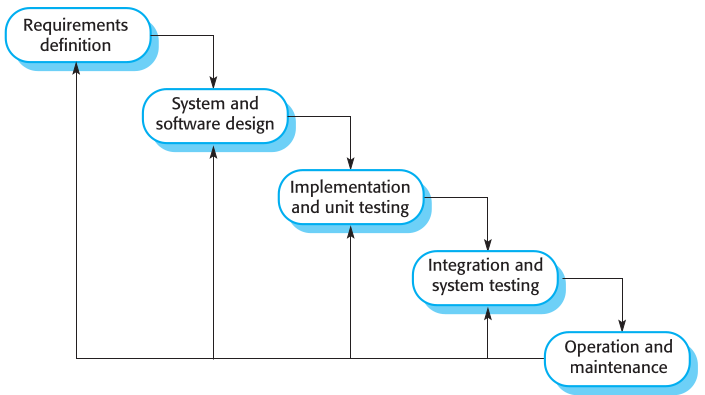
\includegraphics[width=10cm]{\imagesPath/waterfall.png}
    \caption{The waterfall model. From \cite{}}
    % book: figure 2.1 p.47
\end{figure}

Negative
\begin{itemize}
  \item Bad when requirements change quickly.
  \item Not flexible.
  \item May delay the development process when waiting for customer approval.
\end{itemize}

Positive
\begin{itemize}
  \item Well documented.
  \item Often more stable systems.
\end{itemize}

Used in
\begin{itemize}
  \item Embedded systems
  \item Critical systems
  \item Large software systems that are part of broader engineering systems developed
by several partner companies.
\end{itemize}

\textbf{Incremental development}
\begin{figure}[!ht]
    \centering
    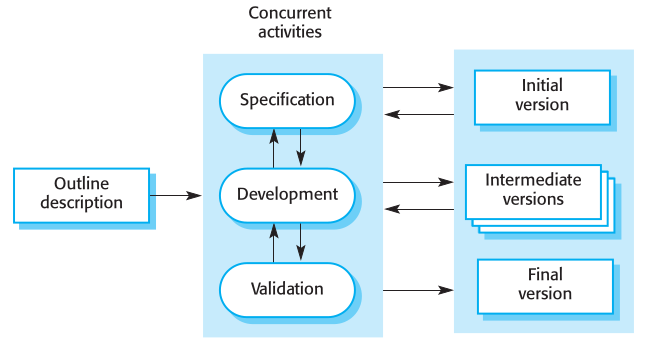
\includegraphics[width=11cm]{\imagesPath/incremental_development.png}
    \caption{Incremental development model. From \cite{}}
    % book: figure 2.2 p.50
\end{figure}

Negative
\begin{itemize}
  \item More difficult and time consuming to messure progress.
  \item Often the system structure degrades as new incroments are developed. Therefore, regular refactoring is needed.
\end{itemize}

Positive
\begin{itemize}
  \item Cheaper than waterfall.
  \item Easier to get feedback from cusomers since one can show a demonstration not just software design documents.
  \item Earlier deliveri and deployment, since a functional version of the software exist.
\end{itemize}

Used in
\begin{itemize}
  \item In software which requirment is likely to change during the development process, which is the case for most buissnesses.
\end{itemize}


\textbf{Integration and configuration}
\begin{figure}[!ht]
    \centering
    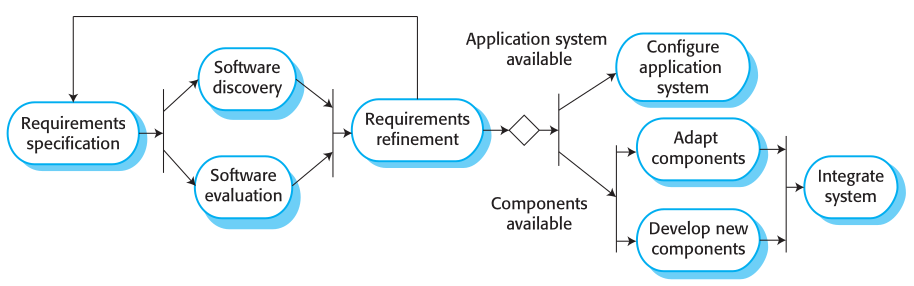
\includegraphics[width=12cm]{\imagesPath/integration_and_configuration.png}
    \caption{Integration and configuration model. From \cite{}}
    % book: figure 2.3 p.52
\end{figure}

Negative
\begin{itemize}
  \item May compromise requirments and therefore, not satisfaing the real needs of the costumer.
  \item System evolotion can be more difficult when the components are not controled by the organization.
\end{itemize}

Positive
\begin{itemize}
  \item Redusing the development of new software and therefore, reducing the cost and risks.
  \item Often faster delivery.
\end{itemize}

Used in
\begin{itemize}
  \item When cost and time is limited.
\end{itemize}

\subsubsection{Process activities}
The four basic process activitest for a software processes are: Software specification, Software design and implementation, Software validation, and Software evolution.

\begin{figure}[!ht]
    \centering
    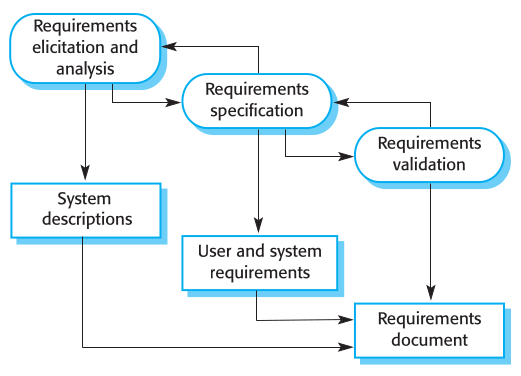
\includegraphics[width=12cm]{\imagesPath/requirements_engineering_process.png}
    \caption{Software specification. From \cite{}}
    % book: figure 2.4 p.55
\end{figure}
\begin{figure}[!ht]
    \centering
    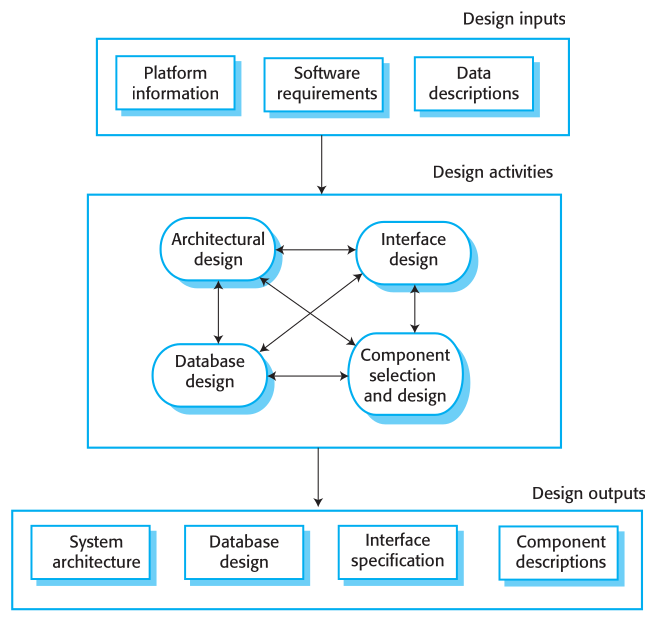
\includegraphics[width=12cm]{\imagesPath/design_process.png}
    \caption{Software design and implementation. From \cite{}}
    % book: figure 2.5 p.56
\end{figure}
\begin{figure}[!ht]
    \centering
    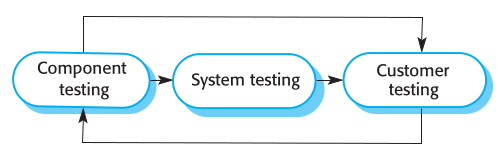
\includegraphics[width=12cm]{\imagesPath/stages_of_testing.png}
    \caption{Software validation. From \cite{}}
    % book: figure 2.6 p.58
\end{figure}
\begin{figure}[!ht]
    \centering
    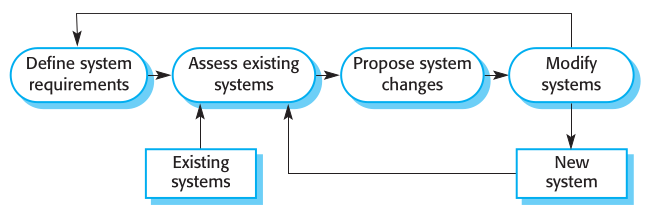
\includegraphics[width=12cm]{\imagesPath/software_system_evolution.png}
    \caption{Software evolution. From \cite{}}
    % book: figure 2.7 p.61
\end{figure}


\subsection{Agile software development}
Agile methods are used to reduse process overhead and documentation, and
increase increments software delivery.

A combination of plan-driven and agile may be used, but they can be used
separately depending on the software being developed.

\textit{User stories} are used to define the customer requirements to
undestand what needs to be done. From these, \textit{tasks} are created
to concretize the work.

\textit{Test-first development} requires the tests to pass before presiding
to the next step. The test are created from a specific tasks.
One issue with this method is ``test-lag'', in other words
when the pace of the developer are faster than the testers.

Introducing agile methods to a organization, which does not have that culture,
is preferably done with a motivated them, which can then spread the methods
across the organization.

Agile methods also produce some issues, e.g. lack of product documentation,
too much work for customers witch may lead to difficulties of customer involved,
and problems with continuity of the development team.

\subsubsection{Agile development practise}
\begin{enumerate}
\item Incremental development
\item Customer involvement
\item Pair programing
\item Regular system releases to customers
\item Refactoring
\end{enumerate}

\subsubsection{Scrum}
\textit{Scrum} provides with a framework of agile methods to easy the management of
project. 

The one who defined the requirments is called the \textit{Product owner}.
It is the task of the \textit{ScrumMaster} to make sure that \textit{Development team}
furfill this requirements. This is done with \textit{Sprint}, which is to process of
development. It used \textit{Product backlog} to define the tasks. The estimate of the size
of the product backlog for a single spring is called \textit{Velocity}.


\begin{figure}[!ht]
    \centering
    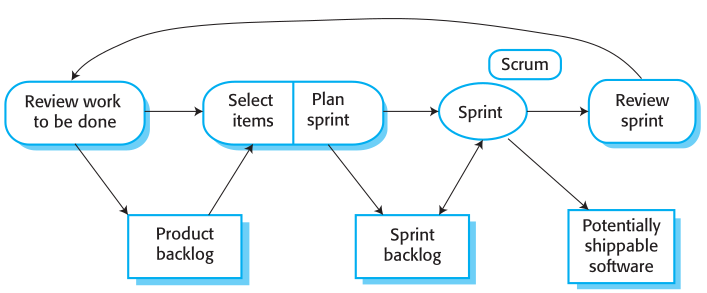
\includegraphics[width=12cm]{\imagesPath/scrum_sprint_cycle.png}
    \caption{Scrum sprint cycle. From \cite{}}
    % book: figure 3.9 p.86
\end{figure}



\subsubsection{Scale agile methods}
Plan-based practices needs to be used with agile practices.
The plan based precesses includes specifying the requirements initially
and provide more documentation. Also, more coordination between teams are required,
such as alignment of realizes, and common tools used in the development.


\subsection{Requirements engineering}
\subsubsection{Functional and non-functional requirements}
\textit{Functional requirements} are specific description on what the system should do.
On the other hand \textit{non-functional requirements} does not describe a necessary
for the service to work for the end user. It is concern is with properties such as:
\begin{itemize}
\item \textit{speed} measured by processed transactions, response time, Screen refresh time.
\item \textit{size} measured by megabytes on disk.
\item \textit{Ease of use} measured by training time.
\item \textit{Reliability} measured by mean time to failure, rate of failure occurrence.
\item \textit{Robustness} measured by time to restart after failure, percentage of events cause failure.
\item \textit{Portability} measured by number of target systems.
\end{itemize}

\subsubsection{Requirements engineering processes}
\begin{figure}[!ht]
    \centering
    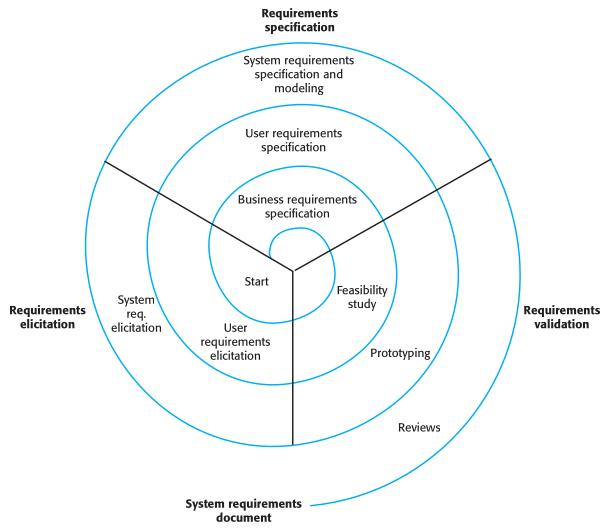
\includegraphics[width=12cm]{\imagesPath/requirements_engineering_processes.png}
    \caption{Scrum sprint cycle. From \cite{}}
    % book: figure 4.6 p.112
\end{figure}


\subsubsection{Requirements elicitation}
\textit{Requirment elicitation} aims to understand the work and processes of the stakeholder
to design the system for them and there needs. From this experiance, requirments can be constructed.

Some techniques are:
\begin{itemize}
\item \textit{Interviewing} which has two types
  \begin{itemize}
    \item Closed interviews
    \item Open interviews
  \end{itemize}
  However, begining with closed questions and then letting openended answers and discussions arise is often more preferable.
\item \textit{Ethnography} is an observation teqniqe in order to study the stakholders day-to-day work. 
\end{itemize}

\textit{Stories} and \textit{scenarios} are also usfull to construct to understand the complete workflow
of the designing system.

\subsubsection{Requirements specification}
The different ways to specify a requirement are
\begin{itemize}
\item \textit{Natural language sentences}
\item \textit{Structured natural language}
\item \textit{Graphical notations}
\item \textit{Mathematical specifications}
\end{itemize}
  
\subsubsection{Requirements validation}
Requirement validation is the process of determineng if the requirements are good or not.
A number of checks can be maid to validate this:
\begin{itemize}
\item \textit{Validity checks}
\item \textit{Consistency checks}
\item \textit{Completeness checks}
\item \textit{Realism checks}
\item \textit{Verifiability}
\end{itemize}
 
\subsubsection{Requirements change}
It is inevitable that requirments changes. Requirements management is the process of controlling and managing these changes.


\subsection{System modeling}
System models are used to make a abstract represenation of the system.

\begin{itemize}
\item \textit{Context models}
  \begin{itemize}
    \item Activity diagrams, shows the activities in the process. See~\ref{activity_diagram}.
  \end{itemize}
\item \textit{Interaction models}
  \begin{itemize}
  \item Use case diagrams, shows the interactions of the user. See~\ref{use_case_diagram}
  \item Sequence diagrams, shows the interaction between the user and the different objects of the system. See~\ref{sequence_diagram}
  \end{itemize}
\item \textit{Structural models}
  \begin{itemize}
    \item Class diagrams, shows how the structure and inheritance of the classes for OOP development. See~\ref{class_diagram}
  \end{itemize}
\item \textit{Behavioral models}
  \begin{itemize}
    \item State diagrams, shows how the system reacts to internal and external events. See~\ref{state_diagram}
  \end{itemize}
\end{itemize}

\begin{figure}[!ht]
    \centering
    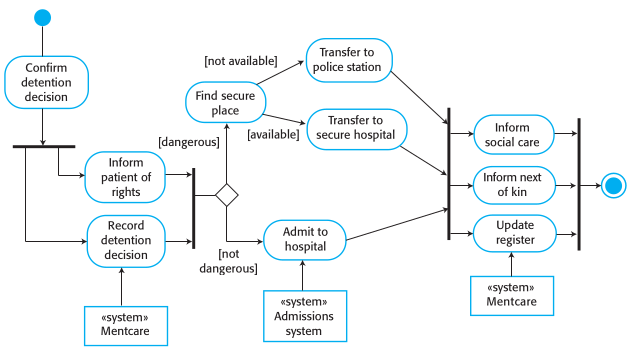
\includegraphics[width=12cm]{\imagesPath/activity_diagram.png}
    \caption{Activity diagram. From~\cite{}}\label{activity_diagram}
    % book: figure 5.2 p.143
\end{figure}
\begin{figure}[!ht]
    \centering
    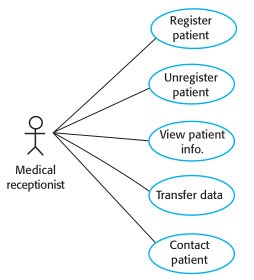
\includegraphics[width=8cm]{\imagesPath/use_case_diagram.png}
    \caption{Scrum sprint cycle. From~\cite{}}\label{use_case_diagram}
    % book: figure 5.5 p.146
\end{figure}
\begin{figure}[!ht]
    \centering
    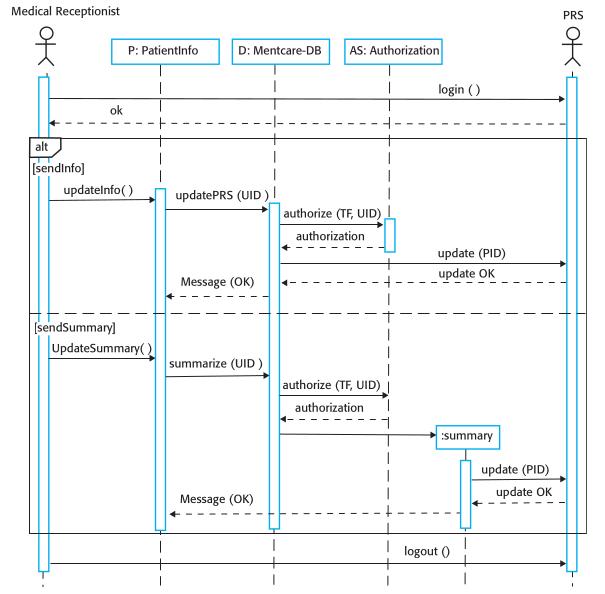
\includegraphics[width=12cm]{\imagesPath/sequence_diagram.png}
    \caption{Scrum sprint cycle. From~\cite{}}\label{sequence_diagram}
    % book: figure 5.6 p.147
\end{figure}
\begin{figure}[!ht]
    \centering
    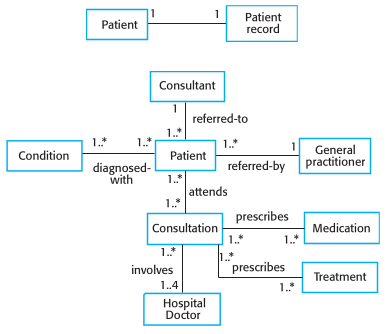
\includegraphics[width=12cm]{\imagesPath/class_diagram.png}
    \caption{Scrum sprint cycle. From~\cite{}}\label{class_diagram}
    % book: figure 5.10 p.151
\end{figure}
\begin{figure}[!ht]
    \centering
    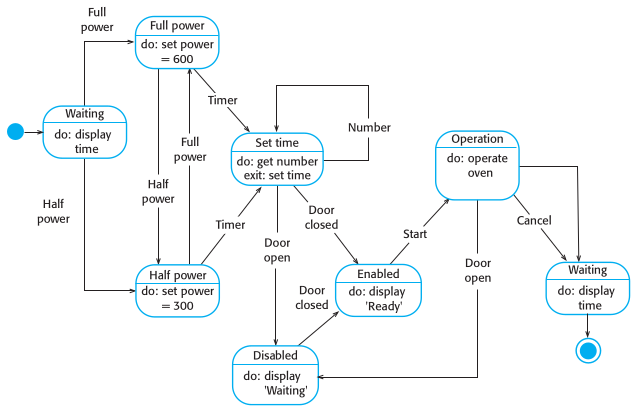
\includegraphics[width=12cm]{\imagesPath/state_diagram.png}
    \caption{Scrum sprint cycle. From~\cite{}}\label{state_diagram}
    % book: figure 5.10 p.151
\end{figure}


\subsection{Architectural design}
Architectural design decisions one has to consider is performance, security, safety, availability, and maintainability. 

The Architectural views are logical view, process view, development view, and phisical view. %(174)

There are severla Architectural patterns, which can be shousen dependent on the system.
MVC, layered architecture, Repository architecture, and pip and filter architecture.

Application architectures help us define commonalites with difftern system and thus design similar systems as sutch. Some of this include Transaction processing system, and Language processing system.

\subsection{Software testing}
\textit{Validation} is whether the product is what it is suppose to be.
\textit{Verification} is if the product work properly.


\subsubsection{Development testing}
Unit testing
\begin{itemize}
\item Should test the diffrent states of the object.
\item A automated test consists of three parts: setup, call, and assertion.
\item There is two stratagies for determin which tests to create: Partition testing and Guideline-based testing.
\end{itemize}

Component testing
\begin{itemize}
\item Components are several interacting objects.
\item Interface errors are the most common error in complex systems. These types of tests are best tested with component testing.
\end{itemize}

System testing
\begin{itemize}
\item Testes the system as a hole and the diffrent functionality of the system.
\item The tests are not just from one development team but can be a combination of diffrent teams.
\item Ofter there exist a dedicated system tester.
\item A sequens of operations makes up a system test.
\end{itemize}


\subsubsection{Test-driven development}
Test-driven development (TDD) is a approch were the tests are first developed and then the implementationof the system. This approach has often better test coverage and is simpler to debugg.

\subsubsection{Release testing}
Is the process of testing realeses, whith a focus on validation.

\textit{Requirements-based testing}, is to validate and verify the requirments is furfilled.

\textit{Scenario testing}, test a use case of the system. It is generaly good to test the combinations
of requirements.

\textit{Performance testing}, is good to test non-functional requirments of preformans. Stress test can also be usfull.


\subsubsection{User testing}
\begin{itemize}
\item Alpha testing, a selected group test that work closely with with the developers give feedback. 
\item Beta testing, a realese that is made avalible for a large group.
\item Acceptance testing, where the customer test if it is ready to be deployed ub the customer enviroment.
\end{itemize}




\section{Part 2 System Dependability and Security}

\section{Part 3 Advanced Software Engineering}
\section{Part 4 Software Management}
